Decision tree algorithm is a very popular way to design a predictive modeling. Decision tree builds classification or regression models in the form of a tree structure. It breaks down a data set into smaller and smaller subsets while at the same time an associated decision tree is incrementally developed. The final result is a tree with decision nodes and leaf nodes. A decision node (e.g., Outlook) has two or more branches (e.g., Runs, Wickets and Run-Rate). Leaf node (e.g., Result) represents a classification or decision. The topmost decision node in a tree which corresponds to the best predictor called root node. Decision trees can handle both categorical and numerical data. Decision tree built on the calculation of Entropy and Information gain.

\section{Entropy Calculation}
Entropy is a measure of unpredictability and uncertainty of a data-set. Entropy is generally considered to determine how disordered a data-set is. The higher rate of entropy refers to the uncertainty and more information needed in these cases to improve the predictability. One outcome is very much certain when the entropy is zero.

\begin{align}
    Entropy(S) &= \sum_{i=1}^{C} Pi \log_{2} Pi 
\end{align}
    
Where Pi is the proportion of instances in the data set that take the i-th value of target attribute, which has C different values. This probability measure give us the idea of how uncertain we are about the data. We use a log2 measure as this represents how many bit we would need in order to specify what the class is of a random instance.

\section{Information Gain}
Now we want quantitative way of splitting the data-set by using a particular attribute. We can use a measure called Information Gain, which calculates the reduction in entropy that would result in split-ting the data on an attribute, A. Information Gain is actually a procedure to select the particular attribute to be a decision node of a decision tree.

\begin{align}
   Gain(S, A) &= Entropy(S) - \sum_{\upsilon \epsilon A} \frac{S_{\upsilon}}{S} Entropy(S_{\upsilon})
\end{align}

where v is a value of A, Sv is the subset of instances of S where A takes the value v and S is the number of instances With the help of this node evaluation technique we can proceed recursively through the subset we create until leaf nodes have been reached throughout and all subsets are pure with zero entropy. This is how a decision tree algorithm works.

\section{Data Training}
After collecting the data we converted those data into an attributed relation file format (.arff) and then we have used Weka for classification. After classification using some algorithm we got some result and later we have analyzed those result. Here is the simple work flow chart given. 

\begin{figure}[ht]
\centering
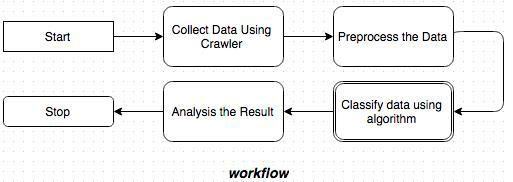
\includegraphics[scale=0.5]{images/fig-5.jpg}
\caption{Workflow}
\label{fig:x Workflow}
\end{figure}


\nomenclature{$\upsilon$}{Upsilon}
\nomenclature{$\epsilon$}{Epsilon}
